\chapter{Querying and Validating Information for GDPR Compliance}
\label{chapter:testing}
% chapter introduction
This chapter presents the application of semantic web technologies to query and validate information for GDPR compliance.
In this, information is represented using the developed vocabularies of GDPRtEXT, GDPRov, and GConsent presented in \autoref{chapter:vocabularies}.
The queries are represented using SPARQL - a W3C standard for querying RDF - and are based on the compliance questions presented in \autoref{sec:info:compliance-questions}.
Validation is carried out based on the identified assumptions and constraints presented in \autoref{sec:info:constraints} and is expressed using SHACL which is the W3C standard for representing constraints.
The presented work represents minor contributions of this thesis, and fulfils the research objective $RO4$ regarding querying of information and $RO5$ regarding validation of information for GDPR compliance.

\autoref{sec:testing:sparql} presents the use of SPARQL to query information for answering compliance questions.
The use of SHACL to validate information for GDPR compliance is presented in \autoref{sec:testing:shacl}.
The chapter ends with conclusions drawn from the research in terms of novelty of contributions in \autoref{sec:testing:conclusion}.

\section{Querying Information for GDPR Compliance using SPARQL}\label{sec:testing:sparql}
This section presents the creation and utilisation of SPARQL queries to retrieve information relevant for GDPR compliance.
The creation of the queries is dependant on the ontological representation of information being retrieved, which in this case includes the use of GDPRov and GDPRtEXT ontologies.
As no consent instances needed to be represented, GConsent was not used.
 This is further explained in \autoref{sec:testing:sparql:relation}.
A GDPR preparation guide published by the Irish Data Protection Commission was used as the source of compliance questions for which corresponding the SPARQL queries were created. The methodology used for this is presented in \autoref{sec:testing:sparql:methodology} with a demonstration of the developed queries presented in \autoref{sec:testing:sparql:demo}.
A note on the evaluation of this work is presented in \autoref{sec:testing:sparql:evaluation}.

\subsection{SPARQL queries and ontological representation of information}\label{sec:testing:sparql:relation}
The research regarding querying presented here is based on the task of retrieving information for answering questions relevant to the assessment of compliance.
It represents utilisation of technical solutions to automate the task of information retrieval and requires machine-readable data (or metadata).
For this, the developed vocabularies provide the ontological concepts and relationships necessary to express the information using GDPR terminology and enable the association of information with clauses and concepts of GDPR.

The compliance questions, as presented in \autoref{sec:info:compliance-questions}, do not use a specific ontology or vocabulary but instead are based in the natural language and use legal terminology. In order to utilise technological solutions for answering them, it is necessary to first convert these questions into queries which can be executed over the compliance representation.
Since the work presented in this thesis derives motivation from the use of semantic web technologies which use RDF for representing information, the task of querying utilises the SPARQL standard to retrieve this information.

The ontology used in the SPARQL queries must match the ontology used in the representation of information associated with compliance. Differences in ontologies would hamper the effective execution of queries with potential returning of invalid results or empty results.
The creation of SPARQL queries is therefore specific to the ontologies used in a particular information representation.

\subsection{Methodology}\label{sec:testing:sparql:methodology}
The methodology used for creation of SPARQL queries is based on utilisation of GDPRov to represent the concepts and GDPRtEXT to link the information to the GDPR.
The SPARQL queries thus created aim to retrieve information relevant to answering the question rather than present an evaluation or assessment of compliance.
While the compliance questions presented in \autoref{sec:info:compliance-questions} provide a basis for construction of semantic queries using SPARQL, the application of SPARQL utilises a real-world use-case of compliance questions to provide a demonstration of the application of this research.

\subsubsection{Utilising compliance questions from GDPR readiness guide published by DPC}
The application of SPARQL utilised the guide titled ``Preparing Your Organisation for the GDPR – A Guide for SMEs'' published by Data Protection Commission of Ireland (DPC) as the basis for compliance questions which were represented using SPARQL as semantic queries.
The guide was published by the DPC in 2017 to help organisations in assessing their readiness towards GDPR compliance requirements.
It is accessible online\footnote{\url{http://gdprandyou.ie/wp-content/uploads/2017/12/A-Guide-to-help-SMEs-Prepare-for-the-GDPR.pdf}} and consists of a `table' (see  \autoref{fig:sparql:guide}) containing questions regarding information about an organisations processing activities.
The guide was chosen based on its simplicity in terms of questions, its intended use in evaluating information associated with compliance, and the locality of the Irish DPC with respect to the author. 

The guide divides the questions into contextual sections based on addressing specific GDPR articles and obligations.
\begin{figure}[htbp]
\centering
\fbox{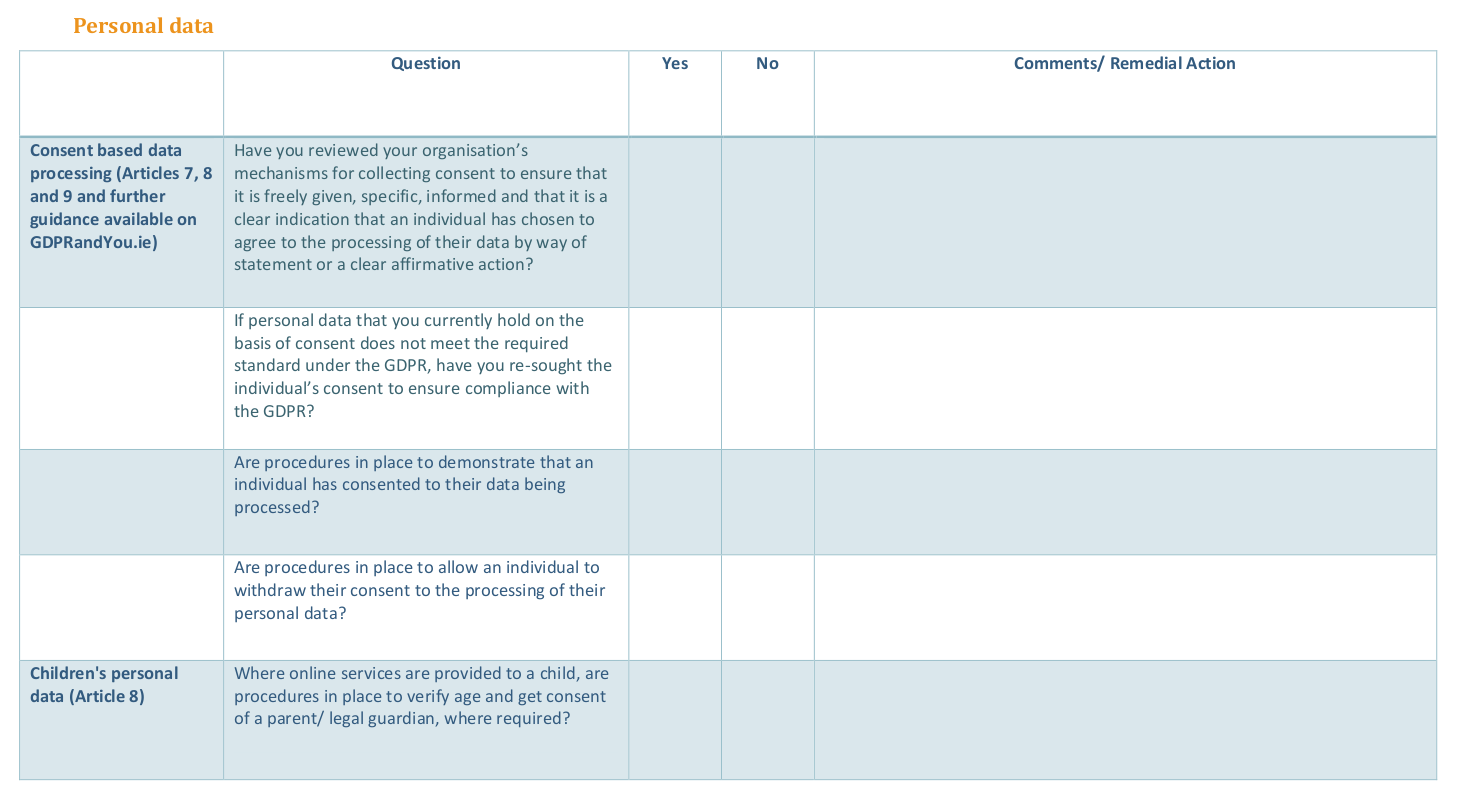
\includegraphics[width=\textwidth]{img/GDPR_guide_page_10.png}}
\caption{Questions for information required to assess compliance - Page 10 of ``Preparing Your Organisation for the GDPR - A Guide for SMEs'' published by Ireland's Data Protection Commission}
\label{fig:sparql:guide}
\end{figure}

\subsubsection{Steps of the methodology}
The steps followed in utilising the questions in the guide to create SPARQL queries and demonstrate their application were as follows:
\begin{enumerate}
    \item Analyse questions within the document to identify corresponding concepts and relationships in GDPRov and GDPRtEXT (see below). The questions largely concerned details of processing activities and organisational practices and therefore did not require use of GConsent.
    \item Represent questions as SPARQL queries using GDPRov and GDPRtEXT (see below)
    \item Create a synthetic use-case based on processing of personal data with GDPRov and GDPRtEXT used to represent information (see \autoref{sec:testing:sparql:demo})
    \item Execute SPARQL queries over use-case to retrieve answers for compliance questions (see \autoref{sec:testing:sparql:demo})
    \item Evaluate the queries based on the subjective criteria of - a) Extent of answering compliance questions b) Suitability of retrieved results in answering compliance questions (see \autoref{sec:testing:sparql:evaluation})
\end{enumerate}

\subsubsection{Analysis of GDPR Readiness Guide}
The guide contains 63 questions across 13 pages that are presented in 9 sections.
Its analysis consisted of categorising the questions based on requirements of information, relation to phases of compliance, and whether they were suitable to be implemented as SPARQL queries.
The analysis was recorded and published online\footnote{\url{https://w3id.org/GDPRep/checklist-demo/notes}} in the form of a spreadsheet with comments describing the thought process in interpreting each question's information requirements.

The first set of questions on page 1 concern consent and personal data and are structurally different than the other set of questions in that they are more abstract and generic and concern the overall practices concerning processing of personal data by the organisation.
These questions are described under the `general' category with other groups of questions having their category mentioned explicitly within the document.
Questions in the general category require information and practices associated with consent and personal data. Other categories contain questions which enquire explicitly about activities and mechanisms regarding compliance to specific obligations.

The questions were analysed and categorised based on their intended requirements towards information required for compliance. The three categories identified through this exercise were - demonstrative, evaluative, and assistive - based on the requirements of information associated with them. 
Demonstrative questions require answers that satisfy the compliance question and do not need further actions or processing based on the information. 
Assistive questions provide information that can be directly evaluated for compliance, with the term `assistive' indicating information that assists in the evaluation.
Evaluative questions retrieve information whose evaluation requires further information retrieved through additional questions based on the provided information.
The primary difference assistive and evaluative questions is whether they retrieve information which can be evaluated as is for compliance or whether it requires additional questions to retrieve further information.
These terms used for categorisation do not relate to any specific methodology used in legal compliance, but are useful to analyse the question from an information management perspective.

Questions were also analysed based on whether they relate to or require information regarding activities in ex-ante and ex-post phases.
The questions do not explicitly provide an indication of whether they enquire about a model of processing (ex-ante) or the execution (ex-post). The distinction was based on whether the question concerned information about practices, plans, or intentions regarding processing of personal data - in which case it was deemed to enquire about ex-ante information.
Similarly, if a question concerned past execution of activities or records of activities - it was said to enquire about ex-post information.
In some cases, questions were specified to enquire about both ex-ante and ex-post information based on potential application in both phases.

An overview of the questions is provided in \autoref{table:sparql:dpc-1}.
It assigns an ID for each question to enable associating it with the corresponding SPARQL query and for linking related questions in the analysis.
The column `\textit{Category}' reflects the category of question mentioned within the guide, with general used for the initial generic questions.
`\textit{Title}' refers to the title of the text within the guide, and the column `\textit{GDPR}' refers to an explicit mention of a GDPR clause within the question or its description.
\begin{center}
\footnotesize
\begin{tabularx}{\textwidth}{|l|l|X|l|}
\caption{Questions provided in the GDPR Readiness Guide} \label{table:sparql:dpc-1} \\
\toprule
\textbf{ID} & \textbf{Category} & \textbf{Title} & \textbf{GDPR} \\
\midrule
\endfirsthead

\caption*{Questions provided in the GDPR Readiness Guide (cont'd)} \\
\toprule
\textbf{ID} & \textbf{Category} & \textbf{Title} & \textbf{GDPR} \\
\midrule
\endhead

\multicolumn{4}{r@{}}{\footnotesize (Cont'd on following page)}\\
\endfoot

% \bottomrule
\endlastfoot

G1 & General & Categories of personal data and data subjects &  \\ \hline
G2 & General & Elements of personal data included within each data category &  \\ \hline
G3 & General & Source of the personal data &  \\ \hline
G4 & General & Purposes for which personal data is processed &  \\ \hline
G5 & General & Legal basis for each processing purpose (non-special categories of personal data) &  \\ \hline
G6 & General & Special categories of personal data &  \\ \hline
G7 & General & Legal basis for processing special categories of personal data &  \\ \hline
G8 & General & Retention period &  \\ \hline
G9 & General & Action required to be GDPR compliant? &  \\ \hline
P1 & PersonalData & Validity of Consent & 7,8,9 \\ \hline
P2 & PersonalData & Retrospective Consent & 7,8,9 \\ \hline
P3 & PersonalData & Demonstration of Consent & 7,8,9 \\ \hline
P4 & PersonalData & Withdraw consent for processing & 7.8.9 \\ \hline
P5 & PersonalData & Children's Personal Data & 8 \\ \hline
P6 & PersonalData & Legitimate interest based data processing &  \\ \hline
R1 & Rights & Subject Access Requests (SARs) & 15 \\ \hline
R2 & Rights & Subject Access Requests (SARs) Response Time & 15 \\ \hline
R3 & Rights & Data Portability & 20 \\ \hline
R4 & Rights & Deletion and Rectification & 16,17 \\ \hline
R5 & Rights & Right to restriction of processing & 18 \\ \hline
R6 & Rights & Right to object to processing & 21 \\ \hline
R7 & Rights & Halt processing after right to object & 21 \\ \hline
R8 & Rights & Profiling and automated processing & 22 \\ \hline
R9 & Rights & Right to obtain human intervention & 22 \\ \hline
R10 & Rights & Restrictions to data subject rights & 23 \\ \hline
A1 & AccuracyRetention & Purpose Limitation &  \\ \hline
A2 & AccuracyRetention & Data minimisation &  \\ \hline
A3 & AccuracyRetention & Accuracy &  \\ \hline
A4 & AccuracyRetention & Retention &  \\ \hline
A5 & AccuracyRetention & Retention Legal Obligations &  \\ \hline
A6 & AccuracyRetention & Destroy data securely &  \\ \hline
A7 & AccuracyRetention & Duplication of records &  \\ \hline
T1 & Transparency & Transparency to customers and employees & 12,13,14 \\ \hline
T2 & Transparency & Provide Information listed in Article 13 & 13 \\ \hline
T3 & Transparency & Provide Information listed in Article 14 & 14 \\ \hline
T4 & Transparency & Provide information when engaging &  \\ \hline
T5 & Transparency & Provide information on facilitating rights &  \\ \hline
C1 & ControllerObligations & Supplier Agreements & 27,28,29 \\ \hline
C2 & ControllerObligations & Data Protection Officers & 37,38,39 \\ \hline
C3 & ControllerObligations & Reasons for not having a DPO & 37,38,39 \\ \hline
C4 & ControllerObligations & Escalation procedures & 37,38,39 \\ \hline
C5 & ControllerObligations & Escalation procedures through a DPO & 37,38,39 \\ \hline
C6 & ControllerObligations & Data Protection Impact Assessments (DPIAs) & 35 \\ \hline
S1 & DataSecurity & Risks involved in processing data & 32 \\ \hline
S2 & DataSecurity & Documented Security Program & 32 \\ \hline
S3 & DataSecurity & Resolving security related issues & 32 \\ \hline
S4 & DataSecurity & Designated individual for security & 32 \\ \hline
S5 & DataSecurity & Encryption & 32 \\ \hline
S6 & DataSecurity & Removing information & 32 \\ \hline
S7 & DataSecurity & Restoring access & 32 \\ \hline
B1 & DataBreach & Documented incident plans & 33,34 \\ \hline
B2 & DataBreach & Regular reviews & 33,34 \\ \hline
B3 & DataBreach & Notifying authorities & 33,34 \\ \hline
B4 & DataBreach & Notifying data subjects & 33,34 \\ \hline
B5 & DataBreach & Documentation of data breaches & 33,34 \\ \hline
B6 & DataBreach & Co-operation procedures for data breach & 33,34 \\ \hline
I1 & InternationalDataTransfer & Data transfer outside EEA & 44,45,46,47,48,49,50 \\ \hline
I2 & InternationalDataTransfer & Special category of Personal Data in Transfer & 44,45,46,47,48,49,50 \\ \hline
I3 & InternationalDataTransfer & Purpose of Transfer & 44,45,46,47,48,49,50 \\ \hline
I4 & InternationalDataTransfer & Transfer Recipients & 44,45,46,47,48,49,50 \\ \hline
I5 & InternationalDataTransfer & Transfer Details & 44,45,46,47,48,49,50 \\ \hline
I6 & InternationalDataTransfer & Legality of international transfers &  \\ \hline
I7 & InternationalDataTransfer & Transparency & \\ \hline
% \bottomrule
\end{tabularx}
\end{center}

\autoref{table:sparql:dpc-2} presents a summarised view of the analysis of compliance questions presented in \autoref{table:sparql:dpc-1}.
The complete information along with additional comments and fields is available in the online published version of the analysis.
In the table, column `\textit{Type}' indicate the type of query based on categorisation as demonstrative, assistive, evaluative based on the description in the sections above.
The column `\textit{Data}' provides information on information required for the question, including results of other queries.
The relation of question to the ex-ante phase of compliance is reflected by the column `\textit{E/A}' and ex-post phase by the column '\textit{E/P}' using boolean \texttt{Y/N} values.
The column `\textit{SPARQL}' indicates whether a SPARQL query was constructed for the corresponding question, with \texttt{N} indicating that a query was not constructed.
The column `\textit{GDPRov}' indicates whether the latest iteration (v0.7) of GDPRov provides the concepts and relationships to answer the compliance question, with a value of \texttt{Y} indicating that it does, \texttt{N} indicating it does not provide that concept, and \texttt{S} indicating the information to be out of scope of the ontology.
Where a query was not constructed, the reason can be inferred by combining the value of \textit{SPARQL} and \textit{GDPRov} columns - for example, where concepts were out of scope for GDPRov the query was not constructed due to lack of concepts. 
% Where a concept was lacking in GDPRov, it was added in a later revision, except in cases where the information could not be modelled due to ambiguity or awaiting legal guidance - such as for data storage periods. 
% The column \textit{GDPRov} therefore indicates whether that question can be represented using SPARQL.
\begin{center}
\footnotesize 
\begin{tabularx}{\textwidth}{|l|l|X|l|l|l|l|}
\caption{Analysis of compliance questions specified in \autoref{table:sparql:dpc-1}} \label{table:sparql:dpc-2} \\
\toprule
\textbf{ID} & \textbf{Type} & \textbf{Data} & \textbf{E/A} & \textbf{E/P} & \textbf{SPARQL} & \textbf{GDPRov} \\
\midrule
\endfirsthead

\caption*{Analysis of compliance questions specified in \autoref{table:sparql:dpc-1} (cont'd)} \\
\toprule
\textbf{ID} & \textbf{Type} & \textbf{Data} & \textbf{E/A} & \textbf{E/P} & \textbf{SPARQL} & \textbf{GDPRov} \\
\midrule
\endhead

\midrule
\multicolumn{7}{r@{}}{\footnotesize (Cont'd on following page)}\\
\endfoot
\endlastfoot

G1 & Demonstrative & personal data, data subjects & Y & N & Y & Y \\ \hline
G2 & Demonstrative & personal data & Y & N & Y & Y \\ \hline
G3 & Demonstrative & personal data, steps that collect data, entities that provide data & Y & Y & Y & Y \\ \hline
G4 & Demonstrative & results of G1, processes acting on data & Y & N & Y & Y \\ \hline
G5 & Demonstrative & results of G4, processes acting on data & Y & N & Y & Y \\ \hline
G6 & Demonstrative & special category personal data & Y & N & Y & Y \\ \hline
G7 & Demonstrative & results of G6, steps that collect data, steps that store data & Y & N & Y & Y \\ \hline
G8 & Not-Implemented & results of G1, steps that store data &  &  & N & N \\ \hline
G9 & Not-Implemented &  &  &  & N & S \\ \hline
P1 & Assistive & consent, steps that acquire consent & Y & N & Y & Y \\ \hline
P2 & Not-Implemented &  &  &  & N & S \\ \hline
P3 & Evaluative & consent & Y & Y & Y & Y \\ \hline
P4 & Evaluative & steps that withdraw consent & Y & N & Y & Y \\ \hline
P5 & Evaluative & steps that acquire consent, steps for age verification & Y & N & Y & Y \\ \hline
P6 & Assistive & steps that process personal data & Y & N & Y & Y \\ \hline
R1 & Assistive & steps that handle SAR & Y & N & Y & Y \\ \hline
R10 & Not-Implemented &  &  &  & N & S \\ \hline
R2 & Assistive & steps that handle SAR & N & Y & N & Y \\ \hline
R3 & Evaluative & steps that address right to data portability & Y & N & Y & Y \\ \hline
R4 & Evaluative & steps that address right to rectification & Y & N & Y & Y \\ \hline
R5 & Assistive & data subject request, steps that process personal data & N & Y & N & Y \\ \hline
R6 & Not-Implemented &  &  &  & N & Y \\ \hline
R7 & Evaluative & steps that process personal data & Y & N & Y & Y \\ \hline
R8 & Assistive & steps that make automated decisions, consent & Y & Y & Y & Y \\ \hline
R9 & Assistive & steps that make automated decisions, right to contest automated decisions & Y & N & Y & Y \\ \hline
A1 & Evaluative & personal data, consent, steps that involve personal data through use, share, store & Y & Y & Y & Y \\ \hline
A2 & Assistive & personal data, steps that process personal data & Y & Y & Y & Y \\ \hline
A3 & Not-Implemented &  &  &  & N & S \\ \hline
A4 & Not-Implemented &  &  &  & N & S \\ \hline
A5 & Not-Implemented &  &  &  & N & S \\ \hline
A6 & Assistive & steps that delete data & Y & N & Y & Y \\ \hline
A7 & Not-Implemented &  &  &  & N & S \\ \hline
T1 & Not-Implemented &  &  &  & N & S \\ \hline
T2 & Assistive & steps that collect personal data & Y & N & Y & Y \\ \hline
T3 & Assistive & steps that collect personal data & Y & N & Y & Y \\ \hline
T4 & Not-Implemented &  &  &  & N & S \\ \hline
T5 & Not-Implemented &  &  &  & N & S \\ \hline
C1 & Not-Implemented &  &  &  & N & S \\ \hline
C2 & Not-Implemented &  &  &  & N & Y \\ \hline
C3 & Not-Implemented &  &  &  & N & S \\ \hline
C4 & Not-Implemented &  &  &  & N & S \\ \hline
C5 & Not-Implemented &  &  &  & N & S \\ \hline
C6 & Assistive & steps part of the DPIA process & Y & N & Y & Y \\ \hline
S1 & Assistive & steps that process data & Y & N & Y & Y \\ \hline
S2 & Not-Implemented &  &  &  & N & S \\ \hline
S3 & Not-Implemented &  &  &  & N & S \\ \hline
S4 & Not-Implemented &  &  &  & N & S \\ \hline
S5 & Not-Implemented & steps that share data &  &  & N & N \\ \hline
S6 & Not-Implemented &  &  &  & N & Y \\ \hline
S7 & Not-Implemented &  &  &  & N & N \\ \hline
B1 & Evaluative & processes or plan that address security incidents & Y & N & Y & Y \\ \hline
B2 & Not-Implemented &  &  &  & N & S \\ \hline
B3 & Evaluative & processes or plans for notifying DPC & Y &  & Y & Y \\ \hline
B4 & Evaluative & processes or plans for notifying data subjects of a data breach &  &  & Y & Y \\ \hline
B5 & Not-Implemented &  &  &  & N & Y \\ \hline
B6 & Not-Implemented &  &  &  & N & S \\ \hline
I1 & Evaluative & steps that share data & Y & Y & Y & Y \\ \hline
I2 & Evaluative & results from I1, category of personal data & Y & N & Y & Y \\ \hline
I3 & Assistive & steps that share data & Y & Y & Y & Y \\ \hline
I4 & Evaluative & steps that share data & Y & Y & Y & Y \\ \hline
I5 & Not-Implemented &  &  &  & N & Y \\ \hline
I6 & Not-Implemented &  &  &  & N & Y \\ \hline
I7 & Not-Implemented & steps that share data &  &  & N & S \\ \hline
\end{tabularx}
\end{center}

% Where the questions could not be answered due to missing concepts and relationships in GDPRov, or due to uncertain interpretations of a legal concept or ambiguity, a note was made to identify solutions in the future.
% This was used to update the GDPRov at a later date with additional concepts, such as for legal bases, data sharing, data transfers, or documentation of data breaches.
The information regarding GDPRov is also provided since the creation of SPARQL queries from GDPR readiness guide was carried out in the earlier stages of GDPRov's iterations and before the enforcement of the GDPR in May 2018. Therefore, some questions were deemed to be ambiguous or lacking legal information on information necessary for compliance.
The queries and constraints presented in \autoref{sec:testing:shacl} were developed at a later stage when GDPR had seen significant attention and interpretation and present a more mature implementation.

\subsubsection{Creation of SPARQL queries}
The creation of SPARQL queries involved analysis of the text of a question to identify relevant concepts and relationships in GDPRov useful towards expressing the question as a semantic query in SPARQL as well as representing the information required to answer the question.
In this, some questions were found to be subjective or qualitative based on the information they required and thus could not be expressed as SPARQL queries. For example, \textit{Question C3} is about reasons for not having a DPO. Such questions are indicated as not implemented in \autoref{table:sparql:dpc-2}.

A total of 33 SPARQL queries were created based on the above analysis of compliance questions and their requirements.
The queries utilised GDPRov and GDPRtEXT ontologies to specify the information associated with the question.
The SPARQL queries were published online\footnote{\url{https://w3id.org/GDPRep/checklist-demo/sparql-queries}}
with separate files for each query associated with a compliance question, and a common file containing the common prefixes used in all queries.

As an example, Listing \autoref{code:sparql:dpc-G5} contains the corresponding SPARQL query for compliance question \texttt{G5} which concerns the legal basis used to justify processing of personal data. 
The query retrieves information about steps and the processes along with the legal basis for their operation in ex-ante phase using the vocabulary provided by GDPRov.
Within this, the query specifically retrieves steps which are defined as being part of a process and use some form of personal data. 
The legal bases can be associated with individual steps or with the process they are associated with.
\begin{listing}[htbp]
\begin{minted}[
    frame=single,
    framesep=5mm,
    baselinestretch=1,
    linenos
]{sparql}
PREFIX rdfs:     <http://www.w3.org/2000/01/rdf-schema#>
PREFIX gdprov:   <http://purl.org/adaptcentre/openscience/ontologies/gdprov#>
PREFIX gdprtext: <http://purl.org/adaptcentre/openscience/ontologies/GDPRtEXT#>

SELECT DISTINCT ?process ?legal WHERE {
  ?data a ?data_type .
  ?data_type rdfs:subClassOf gdprov:PersonalData .
  ?step a ?step_type .
  ?step_type rdfs:subClassOf gdprov:DataStep .
  ?step gdprov:usesData ?data . 
  ?step gdprov:isPartOfProcess ?process .
  OPTIONAL { ?step gdprov:hasLegalBasis ?legal } .
  OPTIONAL { ?process gdprov:hasLegalBasis ?legal } .
} ORDER BY ?process
\end{minted}
\caption{SPARQL query representing compliance question \texttt{G5} concerning legal basis for processing}
\label{code:sparql:dpc-G5}
\end{listing}

\subsection{Demonstration using synthetic use-case} \label{sec:testing:sparql:demo}
To demonstrate the application of queries, a synthetic use-case was created using GDPRov and GDPRtEXT to represent information.
The use-case is based on the scenario of an online shopping service that allows users to order products.
RDF representations of the processes and personal data associated with the use-case were created and queried using the created SPARQL queries to retrieve information regarding compliance.
The implementation was provided online\footnote{\url{https://w3id.org/GDPRep/checklist-demo}} along with its data and code in a public repository\footnote{\url{http://openscience.adaptcentre.ie/GDPR-checklist-demo/demo/}}.
The use-case of an online shopping service is based on its prevalence in the real-world and provides a sufficient representation of purposes, legal bases, processing operations, and third parties involved.
The use-case is intended to provide information for SPARQL to query and as such its complexity does not have a significant bearing on the design of the query itself as long as all the queried concepts have been represented.

\subsubsection{Use-case: Online shopping service that shows ads}
Within the use-case, users can shop for products using the online service i.e. a website. Users have the option to establish an account with the service to receive discounts and special offers for the products offered on the service.
Ads are served to users and are generated by a Third Party.
The sign-up process collects personal data such as name, address, email, and contact number.
While ordering products, users are requested to provide sensitive information for transactions about their bank account or credit cards.

The personal data is represented by sub-classing \texttt{gdprov:PersonalData} as \texttt{CustomerInfo} in the use-case's namespace for representing information about the user.
Similarly \texttt{SensitiveData} is sub-classed for representing banking and financial information as \texttt{gdprov:BankingInfo}.
Processes for handling obligations and rights are expressed using the terms provided by GDPRov.
The sign-up process enables an user to provide information which is used for personalisation and ads and collects the user's consent.
As a final step, the Fact++\footnote{\url{http://owl.cs.manchester.ac.uk/tools/fact/}}
reasoner was used to derive additional facts about the use-case and to ensure its consistency in terms of correct use of GDPRov (and by extension PROV-O and P-Plan) and GDPRtEXT.

\subsubsection{Implementation}
The online demo provides an execution of the created SPARQL queries over the data defined for the use-case.
This represents automation of answering compliance questions using retrieved information.
The demo is intended to showcase how the static GDPR readiness checklist can be made more interactive and automated using semantic web technologies.

The demo is provided as a single web page, with the questions from GDPR readiness checklist provided in their natural language form and ID followed by the corresponding SPARQL query.
The results for each query are retrieved whenever the page loads from a
SPARQL endpoint\footnote{\url{http://openscience.adaptcentre.ie/sparql}}
containing the RDF data about the use-case.
The demo uses the tools YASQE\footnote{\url{http://yasqe.yasgui.org/}} to present SPARQL queries with syntax highlighting and YASR\footnote{\url{http://yasr.yasgui.org/}} to represent the results of queries in an interactive fashion on the web page.

The results of each query contain the information associated with answering the relevant compliance questions. For the SPARQL query regarding question \texttt{G5} presented in Listing. \autoref{code:sparql:dpc-G5} which enquired about legal obligations, the results express the steps and processes along with their legal obligations.
The query and the results as presented in the demo are depicted in \autoref{fig:sparql:demo}.
The results consist of five rows - of which three are processes that handle the various rights and therefore are not accompanied with any legal basis\footnote{The processes handling rights should utilise the legal basis of requirements specified by law since GDPR requires the provision of rights.}.
The remaining two results represent processes associated with the provision of the service, of which \textit{OrderProcess} represents `ordering a product' and uses legitimate interest as its legal basis, and \textit{NewUserSignUpProcess} collects information about an user and uses the legal basis of given consent.
\begin{figure}[htbp]
\centering
\fbox{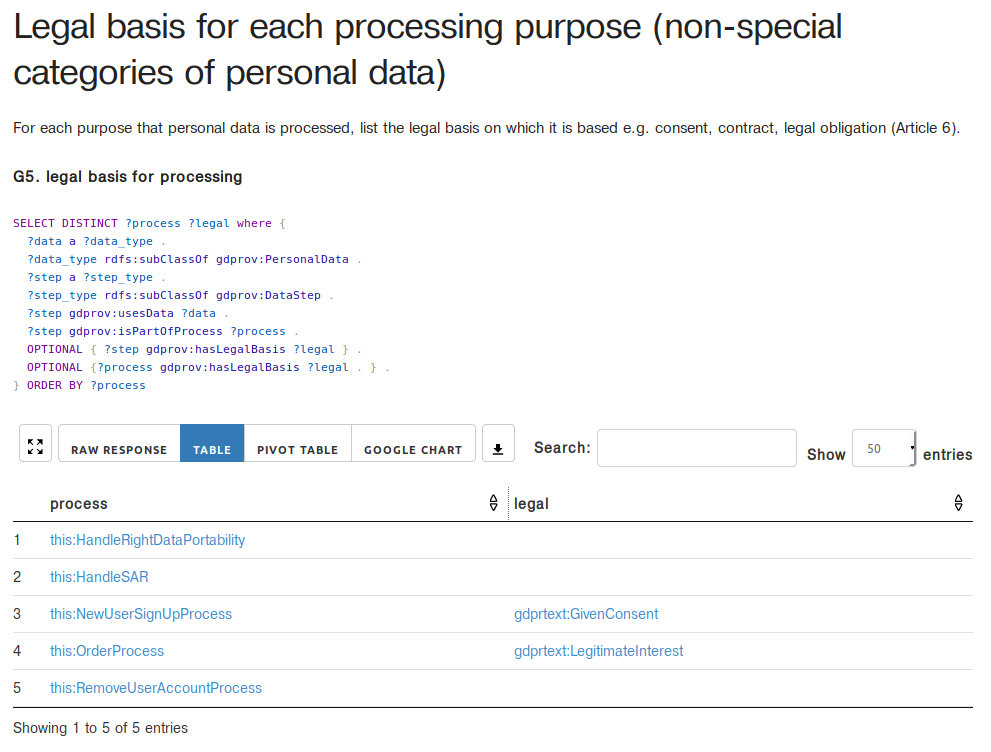
\includegraphics[width=0.75\textwidth]{img/sparql_query_demo.png}}
\caption{Retrieving information using SPARQL for query G5 in GDPR readiness checklist}
\label{fig:sparql:demo}
\end{figure}

\subsection{Evaluation}\label{sec:testing:sparql:evaluation}
The aim of this work was to represent compliance questions using SPARQL in order to retrieve information represented in RDF regarding the processing of personal data.
The demonstration using a synthetic use-case provided the basis for exploring the application of created SPARQL queries by using GDPRov and GDPRtEXT as the ontological representations of data.
The evaluation of this work, while not being exhaustive, demonstrates the creation of SPARQL queries and their application over a given use-case.

In terms of coverage of compliance questions represented as SPARQL queries, the exercise could not represent all of the questions within the GDPR readiness guide.
% Where the reason was GDPRov not providing a required concept, the concept was identified and added to ontology. 
Reasons include a the lack of knowledge regarding representation of ambiguous information such as `indefinite' storage periods and their legal validity, and the query being out of scope for the research question of this thesis.
\autoref{table:sparql:dpc-2} presents an indication of these through the \textit{SPARQL} and \textit{GDPRov} columns.

Since the goal of the exercise demonstrating a questions related to GDPR compliance could be expressed in SPARQL, the evaluation consisted of determining the extent to which this was possible. 
The expression of compliance questions using SPARQL is not novel in itself, as approaches in the SotA present their use of SPARQL in querying information related to GDPR compliance - such as in the SPECIAL, MIREL, and DAPRECO projects.
However, details of their creation and implementation are sparse as pointed out in the SotA analysis in \autoref{sec:sota:analysis}, which makes it difficult to compare the application of SPARQL queries for retrieving information associated with GDPR compliance as presented here in context of the SotA.

Of the total 63 questions within the GDPR readiness guide, 32 questions have corresponding SPARQL queries created and used in the demo.
Of the 31 questions that were not implemented, 20 questions were considered out of scope as they do not relate to the research question, with the other 3 questions lacking corresponding concepts in GDPRov to create SPARQL queries.
Of these, question \texttt{G8} concerning retention periods for personal data can be expressed using the Time ontology \cite{cox_time_2017}.
The other two, \texttt{S5} and \texttt{S7} require specification of information associated with information management and governance procedures utilised within an organisation. While these are technically not outside the scope of GDPRov, they require a larger understanding of how such processes are specified and managed, and commonly involve use of specifications to denote practices, for example ISO/IEC 27001 describing a framework for information management and protection.
Some questions not considered within scope concern information not associated with processing of personal data or consent, but which can be represented as activities using GDPRov. These include questions \texttt{C1} concerning agreements between entities or question \texttt{C4} concerning escalation procedures involving DPO.

The application of SPARQL for querying information associated with GDPR compliance was published in a peer-reviewed publication \cite{pandit_queryable_2018} at the SEMANTiCS conference - which provided its exposure to an audience of industry and academic participants. The publication has received 6 citations to date (excluding self-publications), which includes one approach \cite{debruyneOntologyRepresentingAnnotating2019} which utilises the modelling of concepts using GDPRov towards annotating DFDs (data flow diagrams) with information for analysing compliance, and provides an example of a SPARQL query to retrieve information about the data flows.

% ---------------------------------------------------------------------------------

\section{Validating Information for GDPR Compliance using SHACL}\label{sec:testing:shacl}
This section presents the application of SHACL to validate information based on requirements of GDPR compliance.
SHACL is utilised as a validation mechanism to create a test-driven approach where information regarding processing activities is represented using semantic representations, and is first checked for correctness and then for compliance.
In this, the constraints presented in \autoref{sec:info:constraints} are utilised to determine the correctness and compliance of information, and questions presented in \autoref{sec:info:compliance-questions} are used to retrieve information for compliance.
Both the constraints and the queries are linked to the GDPR using GDPRtEXT.

The results of SHACL validations are persisted to create a `compliance graph' which enables querying for information regarding compliance, and provides more efficient testing based on reuse of ex-ante tests in ex-post testing.
The approach is demonstrated using a proof-of-concept implementation based on the evaluation of consent information on a real-world website and using GDPRov, GConsent, and GDPRtEXT to represent the information.
This approach and the implementation have been published in peer-reviewed publications concerning the conceptual model \cite{pandit_exploring_2018}, construction of a knowledge graph from information about GDPR compliance \cite{pandit_towards_2018}, and implementation testing compliance of given consent on a real-world website \cite{pandit_test-driven_2019}.
All resources regarding this work have been published online\footnote{\url{https://w3id.org/GDPRep/semantic-tests}} under an open and permissive license (CC-by-4.0).

The work presented in this section fulfils the research objectives $RO5$ and demonstrates the following:
\begin{enumerate}
    \item Utilise SHACL to validate information for GDPR compliance.
    \item Express compliance as a test-driven exercise similar to the concept of unit-testing in software engineering.
    \item Utilise results of testing ex-ante information for testing of ex-post information in order to reduce the number of tests required.
    \item Construct a compliance graph storing test results based on the concept of knowledge-graph.
    \item Demonstrate the use of compliance graph in retrieving and documenting information regarding GDPR compliance.
\end{enumerate}

A description of the approach is provided in \autoref{sec:testing:shacl:approach} which presents the role of SHACL as a validation mechanism and the creation of a compliance graph containing information relevant for compliance. The creation of SHACL constraints to represent the natural language constraints in \autoref{sec:info:constraints} is presented in \autoref{sec:testing:shacl:constraints}, with the argument for utilisation of ex-ante validations for evaluation of ex-post information presented in \autoref{sec:testing:shacl:combine}.
A proof-of-concept implementation demonstrating application of the approach is presented in \autoref{sec:testing:shacl:demo}, with the creation of documentation and compliance reports presented in \autoref{sec:testing:shacl:reports}.

\subsection{Validation Model}\label{sec:testing:shacl:approach}
\autoref{fig:shacl:model} presents a visual overview of the approach for the validation model.
The terminology consists of terms utilised by SHACL, with \textit{data graph} indicating the RDF data which is to be evaluated using SHACL, \textit{compliance graph} indicating RDF data containing information relevant for compliance, \textit{completeness} indicating the sufficiency of information i.e. all required data is present, \textit{validation} is the process of evaluating constraints on the data graph, and where \textit{testing} and \textit{evaluating} are used interchangeably with validation as synonyms to refer to the same process.
\begin{figure}[htbp]
    \centering
    \fbox{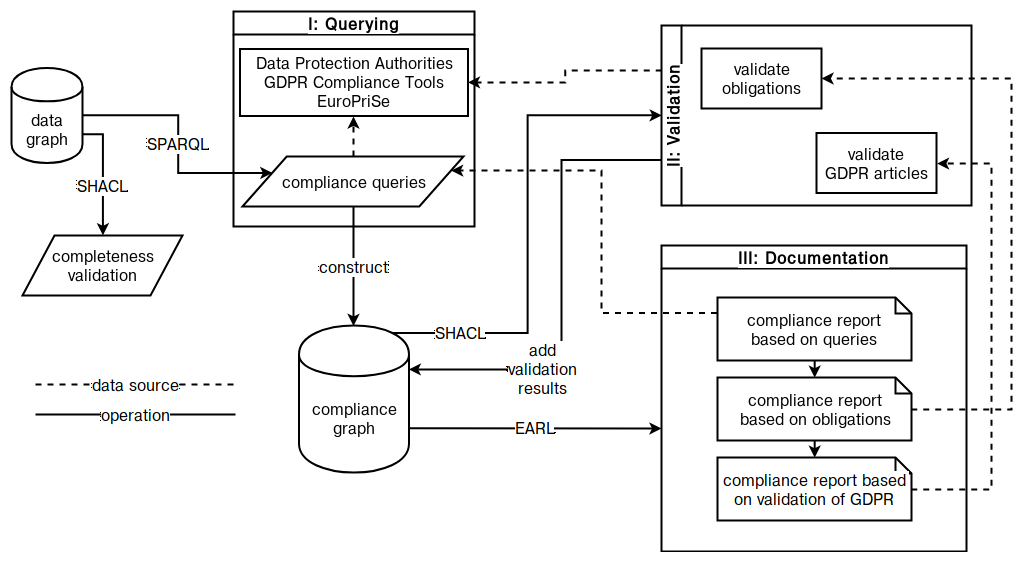
\includegraphics[width=\textwidth]{img/SHACL-model.png}}
    \caption{Overview of approach utilising SHACL to validate information for GDPR compliance}
    \label{fig:shacl:model}
\end{figure}

The approach described in the figure consists of three steps - (i) Querying, (ii) Validation, and (iii) Documentation. A data graph acts as the input and provides information about activities associated with processing of personal data and consent represented in RDF. The data graph needs to be first ensured for `completeness' - i.e. ensuring required information is present before it can be utilised for GDPR compliance.
After this, the first step of querying retrieves information for answering compliance queries by using SPARQL. This information is then added to a `compliance graph' which is separate from the data graph and stores information for determining compliance.

In the second step of validation, SHACL constraints representing obligations and requirements of the GDPR are executed over the compliance graph with the results added back to the compliance graph.
The SHACL constraints and the evaluated results are linked to specific GDPR obligations and articles.
At this point, the compliance graph contains information necessary to answer the compliance questions along with its evaluation using SHACL linked to GDPR.

In the third and final step, the information within the compliance graph is used for documentation of compliance information based on compliance questions, fulfilment of obligations, or coverage of GDPR articles. It queries the compliance graph using SPARQL and retrieves information linked to GDPR.
The results of these can then be persisted or demonstrated using any presentation medium - such as a webpage, dashboard, or even a data file.

The use of RDF makes SPARQL and SHACL the default choices for querying and validation respectively given their status as standards.
However, the model presents a modular approach for querying, validating, and documenting information relevant to compliance. This is to enable the use of alternative technologies for carrying out the tasks associated in a particular step. 
For example, ShEx - another validation standard - can be used in lieu of SHACL to express constraints over RDF data.

The steps only represent a separation of concerns in the description of the model.
In practical uses, such as one presented in this thesis, the first and second steps are combined to consolidate the validations associated with correctness and GDPR obligations.
This is based on the assumption that missing information (which is checked by completeness validations) is a failing condition for the evaluation of compliance.
The constraints presented in \autoref{sec:info:constraints} thus incorporate expression of validations for both completeness and obligations.

\subsection{Creation of SHACL constraints}\label{sec:testing:shacl:constraints}
\subsubsection{Ontologies for expressing SHACL constraints}
\autoref{sec:testing:sparql} mentioned the dependency of SPARQL queries on the underlying data model which necessitated utilisation of the same ontological representations as those used in the information to be queried.
The same argument applies for the validation of information using SHACL, where the constraints must utilise the same ontologies as those used in the RDF it aims to validate.
An alternative is using mapping tables to convert the ontologies used in the data to a common ontology used in the validation constraints - however, this will be a difficult, if not impossible, exercise due to the complexities of finding a common model in all the ontologies that can be potentially used to represent information, such as those within the state of the art.

The constraints presented here use the developed ontologies from \autoref{chapter:vocabularies}, namely GDPRov to represent activities associated with processing of personal data and consent, GConsent to represent information about consent relevant for compliance, and GDPRtEXT to link information with the concepts and clauses of GDPR.
In this, the use of GDPRov and GConsent is complimentary in some of the constraints given their overlap in representing concepts associated with consent.
GDPRtEXT is used to link the constraint to a particular clause within the GDPR to indicate its relevancy regarding compliance. It is also used to link the validation results with clauses in the GDPR to enable querying the results based on GDPR articles, as shown later in \autoref{sec:testing:shacl:reports}.

\subsubsection{Extending SHACL concepts to associate information with GDPR}
In the assessment of information for GDPR compliance, some constraints cannot be evaluated automatically based on their qualitative requirements. For example, constraints associated with given consent that aim to evaluate whether it was `freely given' or `unambiguous'. These constraints need to be manually evaluated and their results require to be stored within the compliance graph.
To distinguish such constraints, the the SHACL concept of \texttt{NodeShape} was extended with a sub-class as \texttt{Constraint} with further sub-classes of \texttt{ManuallyCheckedConstraint} and \texttt{AutomaticallyCheckedConstraint} representing constraints that should be checked manually and automatically respectively. This is presented in Listing.\autoref{code:shacl:manual-constraint}.
The property \texttt{linkToGDPR} was created to link information with the clauses of the GDPR with the range \texttt{eli:LegalResourceSubdivision} to enable associating it with any granular part of the GDPR - such as a chapter, article, paragraph, or sub-paragraph - as GDPRtEXT uses this concept as the parent class of its concepts representing structure of GDPR.
\begin{listing}[htbp]
\begin{minted}{turtle}
:Constraint rdfs:subClassOf sh:NodeShape ;
    rdfs:label "Constraint" .
:AutomaticallyCheckedConstraint rdfs:subClassOf :Constraint, sh:NodeShape ;
    rdfs:label "Automatically Checked Constraint" .
:ManuallyCheckedConstraint rdfs:subClassOf :Constraint, sh:NodeShape ;
    rdfs:label "Manually Checked Constraint" .
    
:linkToGDPR a rdfs:Property ;
    rdfs:range eli:LegalResourceSubdivision ;
    rdfs:label "linkToGDPR" .
\end{minted}
\caption{Extending SHACL \texttt{NodeShape} to express manual and automated checking of constraints}
\label{code:shacl:manual-constraint}
\end{listing}

The constraints utilise both GDPRov and GConsent where appropriate and feasible so as to verify using both ontologies. For example, \autoref{code:shacl:gdprov-gconsent} presents a constraint for checking whether each instance of consent is associated with one and only one Data Subject. In it, the concept of Data Subject could be used from GDPRov or GConsent since they both feature it. Therefore, \texttt{sh:or} in SHACL enables representing the condition where either of those could be used to express a Data Subject.
The constraint is linked to the Article 4-11 of GDPR using the property \texttt{linkToGDPR} mentioned above, and provides a human readable message when the constraint fails using the SHACL property \texttt{sh:message}.
\begin{listing}[htbp]
\begin{minted}{turtle}
:ConsentHasDataSubject a sh:PropertyShape, :AutomaticallyCheckedConstraint ;
    sh:name "Consent --> Data Subject" ;
    :linkToGDPR gdpr:article4-11 ;
    sh:path gc:isConsentForDataSubject ;
    sh:minCount 1;
    sh:maxCount 1;
    sh:or ( [ sh:class gc:DataSubject ] [ sh:class gdprov:DataSubject ] ) ;
    sh:message "Consent should be linked to Data Subject" .
\end{minted}
\caption{SHACL constraint checking Data Subject associated with consent}
\label{code:shacl:gdprov-gconsent}
\end{listing}

\subsubsection{Using SHACL-SPARQL}

SHACL-SPARQL\footnote{\url{https://www.w3.org/TR/shacl/\#shacl-sparql}} is an extension of SHACL core features and provides the use of SPARQL queries to retrieve information failing the associated constraint. \autoref{code:shacl:SHACL-SPARQL} presents alternative representations of the same constraint in SHACL core and SHACL-SPARQL.
The constraint aims to ensure all consent instances have a timestamp.
The SHACL-SPARQL constraint features a SPARQL query that filters instances that have a specified timestamp based on properties provided by GConsent, GDPRov, or PROV-O, while the SHACL core representation uses a \texttt{PropertyShape} to assess the same.
\begin{listing}[htbp]
\begin{minted}{sparql}
# SHACL-SPARQL
sh:select "
    SELECT $this WHERE {
        FILTER NOT EXISTS { $this gc:atTime ?time } .
        FILTER NOT EXISTS { $this prov:generatedAtTime ?time } .
        FILTER NOT EXISTS { $this a gdprov:ConsentAgreementTemplate } .
    } " .
\end{minted}
\begin{minted}{turtle}
# SHACL Core
_:ConsentHasTimestamp a sh:PropertyShape ;
    sh:or (
        [ sh:path gc:AtTime . sh:minCount 1; ] ;
        [ sh:path prov:generatedAtTime . sh:minCount 1; ] ;
        [ sh:path gdprov:ConsentAgreementTemplate . sh:minCount 1; ] ;
    ) .
\end{minted}
\caption{Expressing the same constraint in SHACL-SPARQL and in SHACL core}
\label{code:shacl:SHACL-SPARQL}
\end{listing}

The advantages of using SPARQL queries in SHACL constraints is access to information in instances that fail the validation. This is useful in inserting information about the instance in the test reports, such as the ID or IRI, or even the specific triple that needs correction or verification.
The use of SHACL-SPARQL also allows use of the SPARQL queries from \autoref{sec:testing:sparql} by modifying them to retrieve information that will fail the constraint.

\subsubsection{Validating manually evaluated constraints}
For the manually evaluated constraints represented using \texttt{ManuallyCheckedConstaint}, the result arising from its assessment indicates whether the constraint fails or passes, and is therefore a boolean value.
Therefore, the assessment of manually checked constraints is based on verifying a boolean value associated with the constraint through the SHACL property \texttt{sh:hasValue} which indicates the expected value of a property.
An example of this is presented in \autoref{code:shacl:boolean} which represents a constraint checking whether the given consent was freely given.
The assessment is based on explicitly inserting a triple within the data graph that denotes the manually inspected condition of freely given through the property \texttt{m:consentIsFreelyGiven} whose value must be true to indicate compliance.
The messages of a manually checked constraint are prefixed with \textit{(MANUAL-TEST)} to indicate their qualitative nature in human-intended messages.
\begin{listing}[htbp]
\begin{minted}{turtle}
:ValidconsentIsFreelyGiven a sh:PropertyShape, :ManuallyCheckedConstraint ;
    :linkToGDPR gdpr:article4-11 ;
    sh:name "Consent == Freely Given" ;
    sh:path m:consentIsFreelyGiven ;
    sh:hasValue true ;
    sh:message "(MANUAL-TEST) Consent should be freely given" .
\end{minted}
\caption{Evaluating manually checked constraints using boolean values}
\label{code:shacl:boolean}
\end{listing}

\subsection{Utilising ex-ante test results for ex-post validations}\label{sec:testing:shacl:combine}
Based on distinguishing information about activities in ex-ante and ex-post phases, the constraints will also need to be expressed to evaluate these phases separately.
This will cause duplication of evaluations based on testing of same information across both phases. 
For example, in evaluating whether given compliance is compliant with the requirements of GDPR compliance - which is an ex-post evaluation of compliance - information about criteria such as whether the consent was informed are based on the artefacts shown during the request for consent. The information shown when consent was requested is (usually) part of ex-ante activities and (usually) is common to a large number of consent requests - such as the online consent request form shown to all users on a website. Therefore, the assessment of whether it fulfils the obligations associated with informed consent is also common to all instances of consent based on it. 
By performing an evaluation of this artefact in the ex-ante phase, its (successful) results can be reused for evaluation of all consent based on it in the ex-post phase.
This represents utilisation of ex-ante test results in ex-post validation of a constraint.

The abstraction of this can be summarised based on considering the ex-ante information as that associated with the model or plan of activities, and the ex-post information to be regarding the execution of those activities. Since the model is a common template for all execution of the activities, some of the common ex-ante validations can be performed prior to the execution and the results persisted for use in ex-post validations.
This information, which are expressed as SHACL validation reports for the purposes of this thesis, are persisted in the compliance graph in ex-ante phase validations, and are used as part of the data graph in the ex-post validations.

An example of an ex-post validation incorporating ex-ante test results is presented in \autoref{code:shacl:model-constraint}.
The constraint automatically evaluates the outcome of a previous SHACL validation concerning the given consent model in ex-ante phase indicated by \texttt{sh:ValidationReport} with the property \texttt{sh:conforms} used by SHACL to indicate whether an evaluated data graph has passed or failed the given constraints.
\begin{listing}[htbp]
\begin{minted}{turtle}
:ConsentModelConstraints a sh:NodeShape ;
    sh:targetClass sh:ValidationReport ; 
    sh:property :ValidationReportConforms ;
    rdfs:label "Given Consent following Consent Model constraints" .

:ValidationReportConforms a sh:PropertyShape, :AutomaticallyCheckedConstraint ;
    sh:path sh:conforms ;
    sh:hasValue true ; 
    sh:message "Consent Model should be compliant for given consent to be valid" ; 
    sh:name "Check validation report says data conforms" .
\end{minted}
\caption{Utilising ex-ante test results for consent model in evaluating ex-post instances of given consent}
\label{code:shacl:model-constraint}
\end{listing}

\subsection{Proof-of-concept implementation}\label{sec:testing:shacl:demo}
For a proof-of-concept implementation of the approach, the consent dialogue on the Quantcast\footnote{Web archive snapshot \url{https://web.archive.org/web/20190430014325/https://www.quantcast.com/}} was utilised as a use-case and evaluated for GDPR compliance.
Information from the consent dialogue was manually analysed and represented using GDPRov and GConsent to create the data graph. Additionally, information from other pages on the website were also analysed to identify more information about the purposes, processing, personal data, and third parties mentioned in the consent dialogue.
Resources associated with the implementation are available in a public repository\footnote{\url{https://github.com/coolharsh55/GDPR-semantics-demo/}}.

The choice of use-case was made based on Quantcast being a provider of GDPR consent collection mechanism using the IAB consent framework\footnote{\url{https://advertisingconsent.eu/}} - which is the largest consent framework in use and is based on the collection of consent and sharing of personal information using the internet. The Quantcast website was also one of the few (at the time and to the authors’ knowledge) that allowed changing/withdrawing consent using the same dialogue as the one used to request/provide it.

The aim of this exercise is to demonstrate the use of SHACL in validating information for compliance, and the use of ex-ante test results in validating information in ex-post phase.
It is not intended to act as a compliance evaluation\footnote{The Data Protection Commission of Ireland opened an enquiry on 02-May-2019 into the practices of Quantcast in relation to ``processing and aggregating of personal data for the purposes of profiling and utilising the profiles generated for targeted advertising is in compliance with the relevant provisions of the GDPR'' - source: \url{https://www.dataprotection.ie/en/news-media/press-releases/data-protection-commission-opens-statutory-inquiry-quantcast}. The enquiry was announced well after the completion of the presented work, but bears relevance in terms of its findings - which have not been announced as of yet.} of Quantcast, but serve as a demonstration of the usefulness of technological measures, and particularly the semantic web, in representing, querying, and documenting information for compliance.

\subsubsection{Description of Consent Dialogue}
The consent dialogue, depicted in \autoref{fig:shacl:quantcast-consent-dialogue}, is presented to the user upon visit to the Quantcast website. The consent dialogue consists of multiple pages or panels presenting various abstractions of information and choices which the user can interact with.
The first panel, depicted in the figure as \texttt{(a)}, presents a brief description of processing and purposes and provides an option to provide consent\footnote{Note for clarification: Clicking the `I Accept' button signals consent for all specified purposes, as can be verified by clicking on the `Change Consent' button at the bottom of the page to show the selected choices in the consent dialogue. We avoided the interpretation of qualitative assessments in evaluating whether the "I Accept" button fails consent requirements such as not having options pre-ticked or pre-chosen by default, though we believe this does not satisfy the requirements of valid consent under GDPR. We instead represent these qualitative constraints as \texttt{ManuallyCheckedConstraint} and assume their assessment to always be true.} using the `I Accept' button. Further information is made available through the `Show Purposes' button. Upon giving consent at any stage of the dialogue, clicking the `Change Consent' link in the footer at the bottom of the page shows the consent dialogue with the selected consent choices.
\begin{figure}[htbp]
    \begin{minipage}[b]{0.5\linewidth}
        \centering
        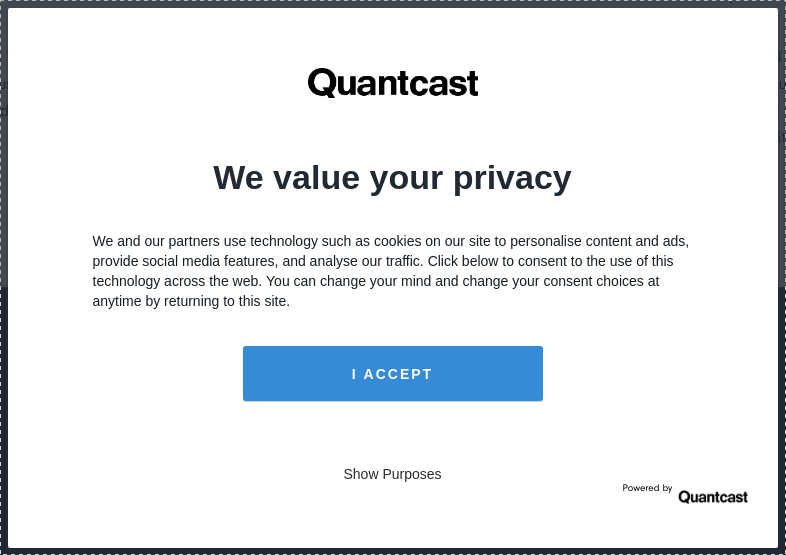
\includegraphics[width=\linewidth]{img/quantcast_consent_screen.png}
        \vspace{0.35cm}
    \end{minipage}
    \begin{minipage}[b]{0.5\linewidth}
        \centering
        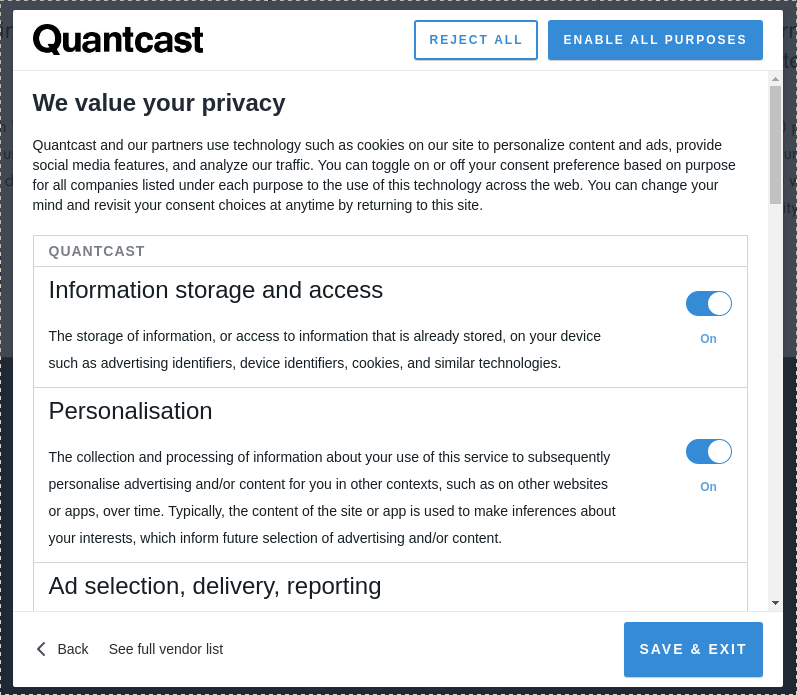
\includegraphics[width=\linewidth]{img/quantcast_consent_I_agree.png}
    \end{minipage}
    \begin{minipage}[b]{0.5\linewidth}
        \centering
        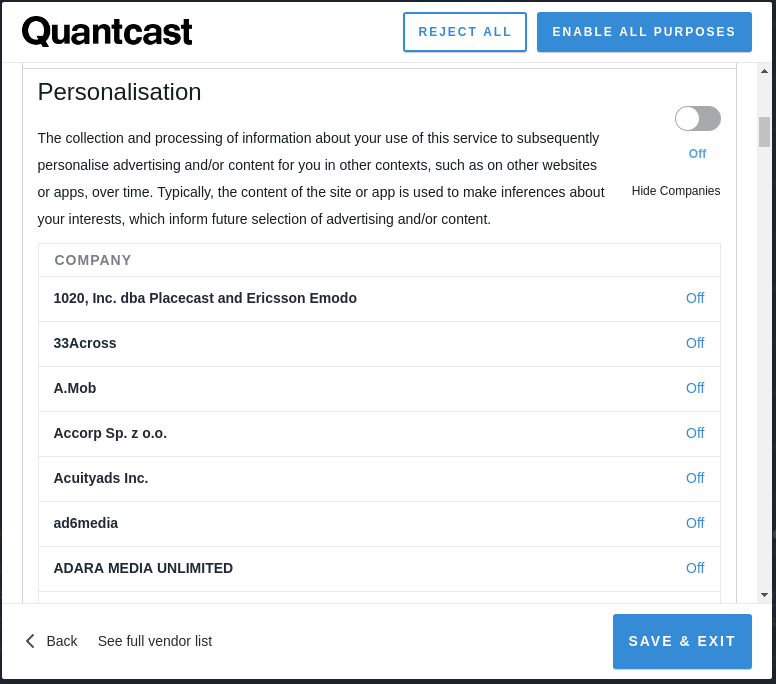
\includegraphics[width=\linewidth]{img/quantcast_third_parties.png}
    \end{minipage}
    \begin{minipage}[b]{0.5\linewidth}
        \centering
        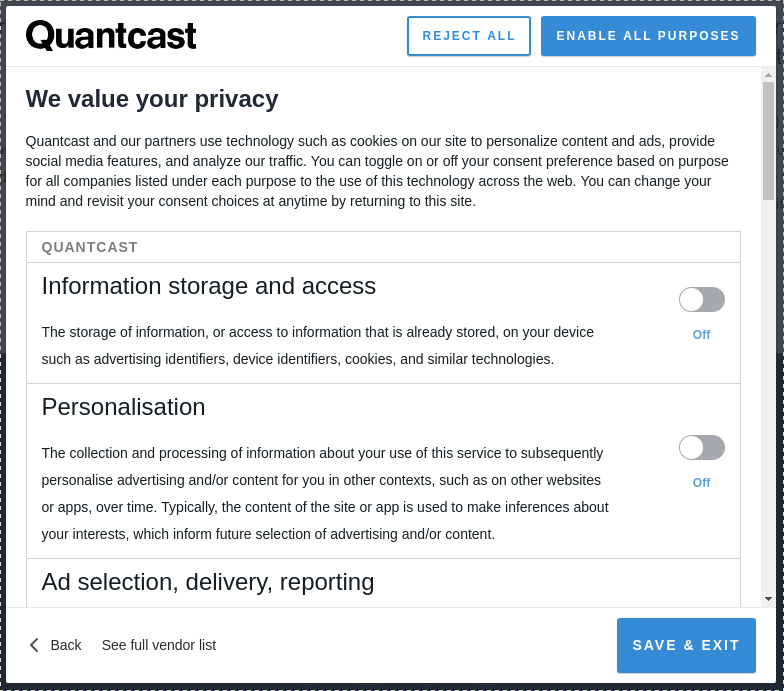
\includegraphics[width=\linewidth]{img/quantcast_consent_info.png}
    \end{minipage}
    \caption{Consent dialogues on \url{quantcast.com} (clockwise from top-left) (a) first screen (b) default options on selecting “I Accept” (c) default options on selecting “Show Purposes” (d) Third parties listed for purpose “Personalisation”}
    \label{fig:shacl:quantcast-consent-dialogue}
\end{figure}

\subsubsection{Extracting Purposes, Processing, and Personal Data from Consent Dialogue}
Clicking the `Show Purposes' dialogue opens the second panel containing information about the  purposes and third parties associated with consent, displayed in figure as \texttt{(b-d)}.
The first section provides information about processing of personal data carried out by Quantcast. Its structuring of information consists of the title specifying the purpose of processing, for example - ``\textit{Information storage}'', followed by a textual description of the persona data categories involved and the processing operations to be performed on them.

The purpose was represented using GDPRov and GConsent as instances of \texttt{gdprov:Process} and \texttt{gc:Purpose} with the title from consent dialogue specified as its label using \texttt{rdfs:label}. 
Information about processing and personal data categories was manually extracted from the text and represented as - \texttt{gdprov:Step} and \texttt{gc:Processing} for processing, and \texttt{gdprov:PersonalData} and \texttt{gc:PersonalData} for personal data.

The consent dialogue was represented using GDPRov as \texttt{ConsentAgreementTemplate} to indicate an ex-ante artefact provided when requesting consent.
Since the consent dialogue offers granular choices from which the user can choose any option individually, the question of its semantic representation leads to two solutions - first where the entire consent dialogue and all consent choices are considered a single instance of consent, and second where each individual and independent choice is considered an instance of consent.
Since given consent for an individual option in the dialogue could be revoked without affecting other choices, each independent option was chosen to be modelled as an instance of consent.
As the consent dialogue acts as a common template for all options, its representation as a `bundle' of consent templates was added to an updated version of GDPRov as \texttt{gdprov:ConsentAgreementTemplateBundle}. This enabled representing a common artefact used to request separate instances of consent.
Listing \autoref{code:shacl:consent-dialogue} provides an example representation of the information from the consent dialogue using this data model.
\begin{listing}[htbp]
\begin{minted}{turtle}
:ConsentRequestDialog a gdprov:ConsentAgreementTemplateBundle ;
    rdfs:label "Consent Dialog shown to the user" ;
    rdfs:comment "Dialog that shows - We value your privacy...
        ... customise their choice by clicking on 'Show Purposes'." ;
    gdprov:usesConsentAgreementTemplate 
        :CATQInfoStorageAccess, :CATQPersonalise, :CATQAds, 
        :CATQMeasure, :CATTPInfoStorageAccess, :CATTPPersonalise, 
        :CATTPAds, :CATTPContentSelection, :CATTPMeasure, :CATTPGoogle .

:CATQInfoStorageAccess a gdprov:ConsentAgreementTemplate, gc:Consent ;
    rdfs:label "consent for CATQInfoStorageAccess" ;
    gc:forPurpose :InformationStorageAccess ;
    gc:forProcessing :StoreIdentifiers, :UseIdentifiers ;
    gc:forPersonalData :Cookie, :AdIdentifier, :DeviceIdentifier ;
    gc:hasLocation <https://quantcast.com/> ;
    gc:withdrawBy <https://www.quantcast.com/#displayConsentUI> ;
    gc:inMedium "dialog box on website" ;
    gc:hasStatus gc:ConsentStatusRequested .
\end{minted}
\caption{Representation of consent dialogue as a bundle of consent requests}
\label{code:shacl:consent-dialogue}
\end{listing}

\subsubsection{Extracting Third-Parties from Consent Dialogue}
In the bottom half of the second panel, the consent dialogue provides information about purposes of sharing data with third parties and a list of recipients for each purpose. This can be seen in the figure in panel \texttt{(c)}.
Consent for each purpose for sharing data with third parties can be individually acted upon by means of a radio button or toggle. Opting to provide consent for a purpose is taken as providing consent for all listed third parties for that purpose, i.e. there is no granular control for consent for individual third parties. 

The third parties were defined using \texttt{gdprov:ThirdParty} and \texttt{gc:ThirdParty}.
Although the names of purposes are the same in sections describing processing by Quantcast (top-half) and by third parties (bottom-half), these were declared as separate instances to reflect separation of choices to provide consent.
Third parties were associated with a particular process by first creating an instance of a data sharing step using \texttt{gdprov:DataSharingStep} and \texttt{gc:DataStep}, and then linking the third party using the property \texttt{gc:SharesDataWithThirdParty}.

\subsubsection{Gathering additional information from Quantcast website}
The consent dialogue does not provide information on how the personal data categories are collected, or the data sources for personal data. To investigate this, an analysis of information about products and services provided Quantcast on their website along with their policies was carried out to identify relevant information which could be added to complete the use-case.

\textit{Measure} is a free service offered by Quantcast that provides analytics regarding audience (visitors) to websites. It uses the following categories of personal data: \textit{Demographics} (age, gender, family, location, income, education, and occupation), \textit{Psychographics} (purchase history, brand preference, cars driven, media consumption), \textit{Engagement} (categorise visitors as passers-by, regulars, and fanatics), and \textit{Traffic} (platform - web and mobile web, country, time period). Of these, data categories of Demographics and Psychographics were included in the data graph as being relevant to the information provided in the consent dialogue. Their source was not indicated by Quantcast and therefore was not added to the data graph.
For Psychographics, Quantcast specifies that it uses information from third-parties (Experian, Mastercard, DLX, TiVo, and Netwise) to `augment' its profiles. The third parties were defined as the the source for this data based on this information.
The profiles mentioned above are described on the webpage as broad categories of data in the form of Shopping Interests, Media Interests, Business \& Occupation, Geography, and Political Interests. These were added to the data graph as personal data categories.

\textit{Targeting} is a service which provides selecting audiences/users based on personal data attributes (similar to those in Measure). While Quantcast\footnote{The service provided by Quantcast is in essence similar to that provided by Facebook - it acts as the mediator between providers and consumers by matching the criteria to user profiles. For example, it mentions an example where the target audience is ``women 18-34 who love shopping, travelling and wine'', which implies that it must know about a) gender b) age range c) website history d) purchase history e) travel history, It further elaborates, ``We build a custom model based on millions of available data points about your audience, such as their pre-search behaviours, demographics, and past purchases.''} does not explicitly say that it uses the same personal data collected and used in Measure, this implication was implicit in its description. However, since this is an assumption, it was not included in the data graph.

\textit{Measurement} is a service similar to Measure and Targeting in its use of audience profile, with the key difference between provision of service beyond website audiences, such as for campaigns. It describes data categories such as Website Traffic, Demographics, Interests, Search behaviours, and Media consumption, which were added to the data graph.

The privacy policy provided by Quantcast provides information regarding personal data categories as Cookies, Tags, and Log data - which were added to the data graph. 
The use and collection of emails used to contact Quantcast were also incorporated.
Data retention periods are provided as ``for as long as necessary'', with an explicit limit for log data provided as 13 months. Due to the ambiguity and pending legal resolution of temporal limits, this information was not added to the data graph.
The privacy policy also described GDPR rights regarding right to access, right to rectify, right to restrict processing, right to deletion, right to data portability, and provided a link\footnote{NOTE: The rights information page could not be accessed in this case with the webpage providing an error regarding Quantcast cookies not being set."} for contact and more information. This link was used as the IRI for activities associated with these rights.

\subsubsection{Validating using SHACL}
As the use-case concerns consent, the constraints associated with consent in \autoref{sec:info:constraints} were used to validate the information using the approach described in \autoref{sec:testing:shacl:approach}.
For evaluation, three sets of constraints were developed to validate: (a) only the ex-ante model of consent dialogue, (b) instances of given consent, and (c) reusing results of ex-ante consent dialogue tests to validate given consent.
This allowed an analysis and comparison of combining ex-ante and ex-post validations, and to demonstrate the benefits in terms of reduced validations and reuse of compliance information.

SHACL constraints were executed using the TopBraid SHACL binary\footnote{\url{https://github.com/TopQuadrant/shacl}}.
A bash\footnote{\url{https://www.gnu.org/software/bash/}} script enabled automation in execution of constraints as different approaches (ex-ante, ex-post, combination of both) and persistence of test results as separate files.

For ease of evaluation, a combined data graph was created consisting of data from Quantcast and the ontologies used - GDPRov, GConsent, GDPRtEXT. 
The data graph and test results were enhanced using a semantic reasoner\footnote{HermiT \url{http://www.hermit-reasoner.com/}} to identify and add additional triples derived from inferences.
The resulting data was added to a triple store\footnote{GraphDB Free Edition \url{http://graphdb.ontotext.com/}} in separate graphs representing the data graph and compliance graph respectively.

\subsection{Generating reports using SPARQL}\label{sec:testing:shacl:reports}
The triple store enabled querying of information to generate compliance reports and documentation.
The use of GraphDB provided access to some in-built reasoning capabilities\footnote{\url{http://graphdb.ontotext.com/free/devhub/inference.html}} which were useful in the querying process.
While a number of SPARQL queries were constructed based on the compliance questions and are available for introspection in the code repository, only one is provided here as an example to demonstrate retrieval of information and documentation of compliance information.

The SPARQL query, listed in Listing \autoref{code:shacl:sparql-report}, retrieves information about each tested validation constraint, its result, link to GDPR, and whether it passed or failed.
The results, shown in \autoref{table:shacl:sparql-report} act as a test report, and contain the constraint description (Name), type - automatic (A) or manual (M), link to GDPR, result - pass (P) or fail (F), and node (instance in data graph) if it failed a constraint.
The report also contains a failure message associated with the constraint that is not shown in table due to space limitations.
\begin{listing}[htbp]
\begin{minted}{sparql}
PREFIX c: <http://example.com/Quantcast/shapes#>
PREFIX sh: <http://www.w3.org/ns/shacl#>
SELECT DISTINCT ?name ?test ?gdpr ?result ?node ?msg
WHERE {
    ?x a c:Constraint .
    ?x sh:name ?name .
    BIND(
        IF(EXISTS{?x a c:AutomaticallyCheckedConstraint},
            "Automatic"^^xsd:string, "Manual"^^xsd:string)
        as ?test)
    OPTIONAL { ?x c:linkToGDPR ?gdpr }
    BIND(
        IF(EXISTS{?y sh:sourceConstraint ?x},
            "FAIL"^^xsd:string, "PASS"^^xsd:string)
        as ?result)
    OPTIONAL {
        FILTER EXISTS { ?y sh:sourceConstraint ?x } .
        ?y sh:focusNode ?node .
    	?y sh:resultMessage ?msg . }
} ORDER BY ?name
\end{minted}
\caption{SPARQL query for report listing validation results linked with GDPR}
\label{code:shacl:sparql-report}
\end{listing}

\definecolor{lightred}{RGB}{255,225,225}

\begin{center}
    \footnotesize
\begin{tabularx}{\linewidth}{|l|X|X|X|l|}
\caption{SHACL validation report linked to GDPR} \label{table:shacl:sparql-report} \\
\toprule
\textbf{Name} & \textbf{Type} & \textbf{GDPR} & \textbf{Result} & \textbf{Node} \\ 
\midrule
\endfirsthead

\caption*{SHACL validation report linked to GDPR (cont'd)} \\
\toprule
\textbf{Name} & \textbf{Type} & \textbf{GDPR} & \textbf{Result} & \textbf{Node} \\
\midrule
\endhead


\midrule
\multicolumn{5}{r@{}}{\footnotesize (Cont'd on following page)}\\
\endfoot

\endlastfoot
    
Consent $\neq$ Inactivity & M & R32 & P &  \\ \hline
Consent $\neq$ Pre-ticked Boxes & M & R32 & P &  \\ \hline
Consent $\neq$ Silence & M & R32 & P &  \\ \hline
Consent $\rightarrow$ Data Subject & A & A4-11 & P &  \\ \hline
Consent $\rightarrow$ Given To & A &  & P &  \\ \hline
Consent $\rightarrow$ Location & A &  & P &  \\ \hline
Consent $\rightarrow$ Medium & A & A7-2 & P &  \\ \hline
Consent $\rightarrow$ Personal Data & A & A4-11,R32 & P &  \\ \hline
Consent $\rightarrow$ Processing & A & A4-11,R32 & P &  \\ \hline
Consent $\rightarrow$ Provided By & A & A7-2 & P &  \\ \hline
Consent $\rightarrow$ Purpose & A & R32,R42 & P &  \\ \hline
Consent $\rightarrow$ Status & A &  & P &  \\ \hline
\rowcolor{lightred} Consent $\rightarrow$ Timestamp & A &  & F & Q:Consent20190415120753 \\ \hline
\rowcolor{lightred} Consent $\rightarrow$ Timestamp & A &  & F & Q:Consent20190415140000 \\ \hline
Consent $\equiv$ Choice & M &  & P &  \\ \hline
Consent $\equiv$ Freely Given & M & A4-11 & P &  \\ \hline
Consent $\equiv$ Specific & M & A4-11 & P &  \\ \hline
Consent $\equiv$ Statement of Clear Action & M & A4-11 & P &  \\ \hline
Consent $\equiv$ Unambigious & M & A4-11 & P &  \\ \hline
Consent Generating Activity & A &  & P &  \\ \hline
Consent Request $\equiv$ Clear & M & R32 & P &  \\ \hline
Consent Request $\equiv$ Concise & M & R32 & P &  \\ \hline
Consent Request $\equiv$ Not Disruptive & M & R32 & P &  \\ \hline
Consent Template & A &  & P &  \\ \hline
Ease of Withdraw Consent & M & A7-3 & P &  \\ \hline
Many Processing x One Purpose & A & R32 & P &  \\ \hline
\rowcolor{lightred} One Processing x Many Purposes & A & R32 & F & Q:Consent20190415120753 \\ \hline
\rowcolor{lightred} One Processing x Many Purposes & A & R32 & F & Q:Consent20190415140000 \\ \hline
\rowcolor{lightred} Personal Data $\rightarrow$ Storage Period & A & A13-2-a & F & Q:CATQInfoStorageAccess \\ \hline
\rowcolor{lightred} Personal Data $\rightarrow$ Storage Period & A & A13-2-a & F & Q:CATTPInfoStorageAccess \\ \hline
\rowcolor{lightred} Personal Data $\rightarrow$ Storage Period & A & A13-2-a,R39 & F & Q:Consent20190415120753 \\ \hline
\rowcolor{lightred} Personal Data $\rightarrow$ Storage Period & A & A13-2-a,R39 & F & Q:Consent20190415140000 \\ \hline
Right to Withdraw & A & A7-3 & P &  \\ \hline
Separation of Processing & M & R43 & P &  \\ \hline
Third Party Categories & A & A44 & P &  \\ \hline
Third Party Identities & A & A13-1-e & P &  \\ \hline
Third Party Identities & A & A30-1-d & P &  \\ \hline
Third Party Identities & A & A44 & P &  \\ \hline
Third Party Safeguards & A &  & P &  \\ \hline
Withdraw Consent Information & M & A7-3 & P &  \\
\bottomrule
\end{tabularx}
\end{center}

The rows which correspond to failed constraints are manually highlighted to provide an indication of the use of information in a visual medium - such as a dashboard.
The query and its results can both be persisted in machine-readable serialisations using standards for representations, making them interoperable and capable of automation.
The information derived from such validations and querying is useful to generate compliance documentation and reports for an organisation to oversee their compliance with the GDPR - which is itself an obligation mandated by the GDPR.

\subsection{Evaluation}
The approach described in \autoref{sec:testing:shacl:approach} for the conceptual model has been published as a peer-reviewed publication \cite{pandit_exploring_2018} in the Poster \& Demo track at the SEMANTiCS conference - which involves a good mix of industry and academic participants and thereby provided the opportunity to present this work to the industry in particular. 
The construction of a knowledge graph based on evaluations of GDPR compliance was published as a peer-reviewed publication \cite{pandit_towards_2018} in the workshop on Contextualized Knowledge Graphs which was co-located with the International Semantic Web Conference (ISWC). The workshop provided reviews and feedback from domain experts regarding the use of semantic web to create knowledge graphs, and how it might be utilise in the legal compliance domain. 
The proof-of-concept implementation presented in \autoref{sec:testing:shacl:demo} was published as a peer-reviewed publication \cite{pandit_test-driven_2019} at the SEMANTiCS conference.

\subsubsection*{Effectiveness of combining ex-ante and ex-post validations}
In order to understand the number of validations in the testing process, consider the set $V_{t}$ consisting of all validations that should be evaluated in order to determine the validity of given consent. This set consists of validations evaluating the information in the consent dialogue box which is common to all instances of given consent - these are represented by $V_{a}$. The remaining validations consist of evaluating information specific to that instance of given consent, such as timestamps, and are represented by $V_{p}$. 
To summarise, the set of validations consists of validations evaluating the consent dialogue and the information within the given consent, with the relation $V_{t} = V_{a} + V_{p}$.

$V_{a}$ is required to be carried out as part of ex-ante compliance evaluations where the organisation must monitor and ensure its activities are compliant before any processing takes place. In this case, the consent dialogue box is required to be evaluated and found compliant before any consent is requested. Therefore, $V_{a}$ represents ex-ante validations and $V_{p}$ represent ex-post validations.

If the results of $V_{a}$ are persisted, then they can be reused in the evaluation of given consent by simply checking whether the outcome of $V_{a}$ was valid or invalid - which is a single validation. Therefore, the total validations to be performed when combining ex-ante and ex-post validations is now $V_{t} = 1(V_{a}) + V_{p}$ - which is efficient assuming $V_{a} > 1$.

In the use-case of consent dialogue presented in this section, $V_{t}=59$ validations of which $V_{a}=57$ validations and $V_{p}=2$ validations. If all validations were evaluated for given consent, each instance of given consent would need $59$ validations. Whereas, if the ex-ante validations were reused and only the ex-post validations were evaluated, then each instance of given consent would need only $3$ validations to be evaluated ($1$ validation to evaluate $V_{a} + 2$ validations from $V_{p}$). While these numbers are use case specific, it clearly demonstrates that the approach is more efficient in terms of validations and determining validity of given consent. This is assuming the ex-ante model of consent dialogue was found compliant in the ex-ante stage, and therefore its validation only evaluated the presence of a test report affirming its compliant status.

\subsubsection*{Comparison with SotA}
\autoref{table:shacl:sota} provides a comparison of the use of SHACL with approaches within the SotA based on the earlier analysis in \autoref{sota:analysis:compliance}.
The SPECIAL project uses a semantic reasoner to determine whether a given combination of processing operations expressed as OWL2 class axioms are valid \cite{westphal_spirit_2018}, while the work presented by Vos et. al \cite{vos_odrl_2019} uses ODRL profiles to express requirements which are converted to and evaluated using Answer Set Programming (ASP).
The MIREL project detects violations of the GDPR by utilising the PrOnto ontology \cite{palmirani_pronto_2018,palmirani_pronto_2018-1,monica_modelling_2018} to model legal concepts and LegalRuleML to model norms, which are then applied over a BPMN use-case using Regorous to generate a report \cite{monica_modelling_2018}.
The DAPRECO project uses PrOnto along with Reified Input/Output logic (RIO) \cite{robaldo_reified_2017} to specify norms and rules to create a knowledge base \cite{bartolini_agile_2019} which is used to compare GDPR with ISO and to determine compliance.
These efforts show the variance in evaluation of compliance and the use of semantic web technologies in evaluation of compliance.
\begin{table}[htbp]
\footnotesize
\centering
\caption{Comparison of SHACL validation with SotA} \label{table:shacl:sota}
\rowcolors{1}{}{gray!10}
\begin{tabularx}{\textwidth}{|l|l|l|X|X|X|}
\toprule
\textbf{Approach} & \textbf{Evaluation method} & \textbf{Scope} & \textbf{Machine-readable result?} & \textbf{Provides remedies?} & \textbf{Links results to GDPR?} \\ 
\midrule
\endfirsthead
\rowcolor[gray]{0.8}
Pandit & SHACL & RDF data & \cmark & \cmark & \cmark \\ \hline
SPECIAL & OWL & Consent & \cmark &  &  \\ \hline
SPL+SERAMIS & ODRL & Obligations & \cmark & \cmark & \cmark \\ \hline
SPL+Vos et al. & OWL, ASP & Obligations & \cmark & \cmark &  \\ \hline
SPL+CitySPIN & OWL & Consent & \cmark &  &  \\ \hline
MIREL & RuleML & Obligations & \cmark & \cmark & \cmark \\ \hline
MRL+DAPRECO & RuleML & Obligations & \cmark & \cmark & \cmark \\ \hline
BPR4GDPR & OWL & Process Flows &  & \cmark &  \\ \hline
Lodge et al & SDK & Process Flows & \cmark & \cmark &  \\ \hline
Tom et al & BPMN & Process Flows & \cmark & \cmark &  \\ \hline
Corrales et al & Questionnaire & Obligations &  &  &  \\ \hline
LUCE & Smart Contracts & Data Sharing & \cmark &  &  \\ \hline
AdvoCATE & Smart Contracts & Consent & \cmark &  &  \\ \hline
Sion et al & UML, DFD & Process Flows & \cmark & \cmark &  \\ \hline
privacyTracker & Access Control & Data Sharing & \cmark &  &  \\ \hline
Robol et al & STS & Process Flows & \cmark &  &  \\ \hline
GuideMe & Questionnaire & Process Flows &  & \cmark &  \\ \hline
Basin et al & Algorithm & Process Flows &  &  &  \\ \hline
RestAssured & XACML & Process Flows & \cmark &  &  \\ \hline
DEFeND & Questionnaire & Obligations & \cmark &  &  \\ \hline
OPERANDO & Access Control & Process Flows & \cmark &  &  \\ \hline
PoSEID-on & Smart Contracts & Data Sharing & \cmark &  &  \\ \hline
DECODE & Smart Contracts & Consent & \cmark &  &  \\ \hline
\end{tabularx}
\end{table}

The work described in this section demonstrates how SHACL can be used to validate information for correctness and adherence to obligations mandated by GDPR based on the interpretation of compliance questions from \autoref{chapter:information}. In this form, SHACL can be used to evaluate compliance, though the presented work focused more on the validation of constraints based on the concept of compliance questions.
Compared to the state of the art in \autoref{chapter:sota}, summarised in the above table, the work regarding SHACL (highlighted first row of table) is novel within the SotA in the use of SHACL and the linking of results to GDPR in a machine-readable and thus query-able form.
In addition, the creation of a compliance graph to store information associated with demonstration of compliance enables using SPARQL queries to identify remedial measures to achieve compliance as well as create reports to identify and present information relevant to compliance.
The utilisation of ex-ante test results in ex-post validations is also novel within the state of the art.

In comparison with SHACL, approaches in the SotA provide a more formal approach based in logic where legal norms can be expressed in terms of requirements and evaluated to determine compliance.
In turn, SHACL provides a validation framework where the results can be persisted as a graph and queried. In addition, the SHACL validations can be linked to the GDPR, as demonstrated using GDPRtEXT, which makes it possible to use SHACL to verify the output of other compliance evaluation approaches and record the outcome as a test result linked to GDPR clauses, thereby creating a graph of compliance.
This also provides an opportunity to explore the reuse of existing approaches and resources regarding evaluation of GDPR compliance where SHACL is used to generate an interoperable overview of the evaluation results while abstracting the underlying outputs from various approaches.
For this, the resources provided by Vos et. al \cite{vos_odrl_2019} and DAPRECO project \cite{bartolini_agile_2019} provide constraints expressed using logic-based formalisms and are available as open access, providing future direction for the applicability of this research.

\section{Summary of Chapter}\label{sec:testing:conclusion}

\subsubsection*{Summary of work presented}
\autoref{sec:testing:sparql} presented the use of SPARQL queries for representing compliance queries and retrieving information associated with compliance that was represented using GDPRov and GDPRtEXT ontologies.
The work fulfilled the research objective $RO4$ by representing the compliance questions as SPARQL queries and demonstrating their application using a real-world use-case.
The demonstrated application used questions from GDPR readiness guide published by the Data Protection Commission of Ireland in 2017 to assist organisations in assessing their adherence to compliance requirements of the GDPR.
The created SPARQL queries retrieved information for answering these compliance questions for a synthetic use-case based on the scenario of an online shopping service.
The queries and the demo were published in a peer-reviewed publication \cite{pandit_queryable_2018} at the SEMANTiCS conference and are available online as an application with the resources provided in a code repository.

\autoref{sec:testing:shacl} presented the use of SHACL to validate information regarding its correctness and adherence to obligation towards GDPR compliance.
This work fulfilled the research objective $RO5$ by validating information using SHACL and linking the results with relevant clauses of GDPR for compliance documentation.
The SHACL validation utilised constraints developed from analysis of compliance questions as presented in \autoref{sec:info:constraints}.
An approach for the validation process using SHACL was presented in which ex-ante test results were reused in the validation of ex-post information. This enabled efficient evaluations by reducing the number of validations required in the ex-post phase, and also enabled associating the compliance of ex-ante information with that of its corresponding ex-post information.
A demonstration of the approach was provided through a use-case in which the consent dialogue on a real-world website was represented using the developed ontologies and validated using SHACL.
The results of the validation were queried using SPARQL to generate documentation for compliance in the form of a test report which showed the compliance status of different obligations and highlighted failing tests as action items for meeting compliance requirements.
The approach of using SHACL and the combination of ex-ante and ex-post validations was published in a peer-reviewed publication \cite{pandit_towards_2018} at the SEMANTiCS conference in 2018, while the demonstration was published in a peer-reviewed publication \cite{pandit_test-driven_2019} at SEMANTiCS 2019.
The resources associated with the work have been made available online in a code repository.

This chapter, through both presented works, provides an application of the developed ontologies presented in \autoref{chapter:vocabularies} for querying and validating information about GDPR compliance.
It serves to demonstrate the usefulness of these ontologies, as well as provide an indication of their role in the representation of information.
The chapter also demonstrates the use of semantic web technologies in representing, querying, and validating information for GDPR compliance.

The modular test-based approach can be used with existing representations in non-RDF data that are evaluated using other tools and methods by adding semantics to the test results and reports to link them with relevant information in GDPR. This will enable the utilisation of a validation method such as SHACL to evaluate its correctness and a querying method such as SPARQL to retrieve information in the form of compliance test reports. 

The advantages of representing processes with semantics go beyond testing for compliance as representation of processes are also useful for planning of operations and internal documentation. Semantic representations of processes can assist in automating the generation of documentation such as privacy policies where processes are listed along with their purpose, legal basis, and use of personal data. Privacy policy generators that generate boilerplate policies exist online, but do not currently incorporate semantics. The use of semantics allows queryable machine-readable metadata that can be used in tools towards understanding and evaluating policies for users and authorities.

\subsubsection*{Re-usability of developed resources}
The interpretation of compliance questions in the GDPR readiness document using SPARQL and its application in the synthetic use-case demonstrates the potential application and usefulness of SPARQL queries to retrieve information relevant for compliance.
However, it also showcases that the creation of SPARQL is highly dependant on utilising the same ontological concepts as the data it is querying. Therefore, such SPARQL queries are use-case dependant, and by definition do not have re-usability beyond the data they were created for.
The same is true for the constraints represented in SHACL, which are dependent on the underlying ontologies used to represent the data graph it intends to validate.

Using the analysis and natural language basis of the questions and constraints, another approach can adopt these resources to query and validate information using its use-case specific ontologies.
While the individual query or constraint would need rewriting, the overall approach and modelling of tests can be reused to generate similar compliance documentation.
The provision of all resources under a permissive licenses provides an adopter with access to the underlying data and information to assist them in this process.

\subsubsection*{Novelty of presented work}
The use of SPARQL and SHACL for GDPR compliance as presented in this chapter is novel within the state of the art as presented in \autoref{sec:sota:analysis}.
While approaches in the SotA use SPARQL to query information, none present their work as intended to answer compliance questions or as intended to investigate the compliance of an organisation.
The use of SHACL is a first within the SotA regarding validation of information for GDPR compliance, based on the analysis of approaches in \autoref{sota:analysis:compliance}.
In addition, the work presented in this thesis has been published in peer-reviewed publication with open access to its data and resources for transparency.
Together, these serve as novel contributions that extend the state of the art.
